
\documentclass[11pt]{amsart}
\usepackage[left=2cm,top=2cm,right=2cm,bottom=2cm,nohead,foot=2cm]{geometry}
\geometry{letterpaper}
\usepackage[parfill]{parskip}
\usepackage{graphicx}
\usepackage{amssymb}
\usepackage{amsmath}
\usepackage{float}
\usepackage{epstopdf}
\usepackage{moreverb}
\usepackage{multicol, multirow}
\usepackage{comment}
\usepackage{wrapfig}
\DeclareGraphicsRule{.tif}{png}{.png}{`convert #1 `dirname #1`/`basename #1 .tif`.png}
\DeclareGraphicsExtensions{.pdf,.png,.jpg}
\usepackage{tikzsymbols}


%creating solution environment
\specialcomment{sol}{\textbf{Solution: }}{}
%this command toggles the solutions

%For the lazy:
\newcommand{\ds}{\displaystyle}
\newcommand{\be}{\begin{enumerate}}
\newcommand{\ee}{\end{enumerate}}
\newcommand{\mrm}{\mathrm}
\newcommand{\bee}{\begin{eqnarray*}}
\newcommand{\eee}{\end{eqnarray*}}
\newcommand{\dds}[2]{\frac{\mathrm{d}#2}{\mathrm{d}#1}} %(d1 BY d2)
\newcommand{\ddb}[2]{\frac{\mathrm{d}}{\mathrm{d}#1}\left[ #2\right]}
%(d by d1 OF 2)

\begin{document}

\begin{minipage}{0.5\textwidth}
		\noindent {\bf CSCI 2824 -- Spring 2020}
\end{minipage}\hfill
\begin{minipage}{0.5\textwidth}
		\noindent \hfill {\bf Homework 10}
\end{minipage}
\noindent This assignment is due on Wednesday, Apr 22 to Gradescope by 11:59pm.  You are expected to write up your solutions neatly and \textbf{use the coverpage}.  Remember that you are encouraged to discuss problems with your classmates, but you must work and write your solutions on your own. 

{\bf Important}: On the {\bf official CSCI 2824 cover page} of your assignment clearly write your full name, the lecture section you belong to (001 or 002), and your student ID number.  You may \textbf{neatly} type your solutions for +2 extra credit on the assignment. You will lose \textit{all} 5 style/neatness points if you fail to use the official cover page.

\vspace{5mm}
\be
%==============================================================================
% Counting
%==============================================================================
\item A common ``brainteaser" puzzle asks the following:  suppose we draw an isosceles triangle, and then draw $k$ lines from the central vertex to various unique points on the opposite edge.  Suppose we also draw $n$ unique lines through the triangle, each parallel to the opposing edge.  We are going to count how many distinct triangles have been created.\\ 

For example, the $n=0$ and $k=1$ triangle is shown on the left.  It contains 3 distinct triangles: the outer lines form a triangle, and the left and right sides also form triangles.   The $n=2$, $k=3$ triangle is shown at right.\\

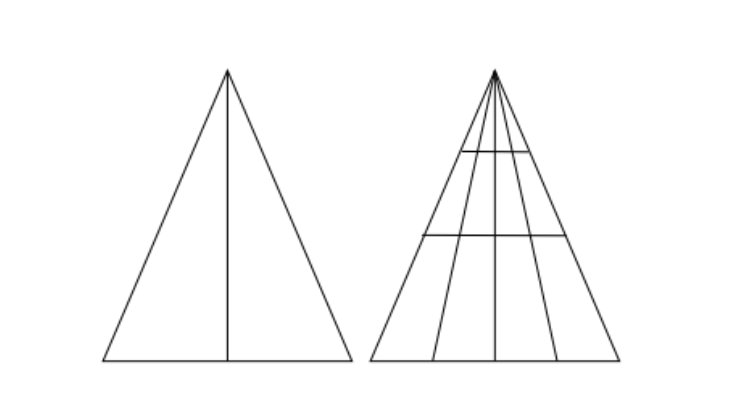
\includegraphics[width=.25\textwidth]{triangles.png}\\

What is the total of number of triangles as a function of $n$ and $k$?  Use a sentence to explain why your result is the case.\\

	\begin{sol}
		\\As you draw more and more vertical lines, the number of triangles increases linearly, in other words:\\
		triangles due to only vertical $= \sum^{k+1}_{n=1} n$\\
		triangles due to only horizontal $= (n+1) \sum^{k+1}_{p=1} p$\\
		\\
		$\therefore$ total triangles $= (n+1)\frac{(k+1)(k+2)}{2}$
	\end{sol}
%==============================================================================
% Probabilty Indepdendence
%==============================================================================
\item Ask yourself: when you draw cards from a deck, does the order matter?  Answer the following:
	\be
	\item You have a standard 52 card deck.  If you draw two cards at random, what is the probability that they are both hearts? 
	
	\item You reshuffle your cards into the deck, but unfortunately now a mischievous dog (a portly Beagle named Lola), decides to eat one of the cards!  Assuming that the missing card is a diamond, now when you draw two cards at random what is the probability that they are both hearts? 
	
	\item Suppose you have your now-51 card deck, and you randomly draw two cards from it.  Both are hearts.  Given this, what is the probability that the missing card is a diamond?
	
	\item Are the events (two cards drawn at random are both spades) and (the missing card is a diamond) independent?  Justify your answer.
	\ee
	\begin{sol}
		\be
			\item $\frac{\binom{13}{2}}{\binom{52}{2}} = \mathbf{0.0588}$

			\item $P$(both are spades / missing card is diamond)\\
			$= \frac{0.0588 \cdot \frac{\binom{13}{1}}{\binom{52}{1}}}{52 \cdot \frac{\binom{13}{1}}{\binom{52}{1}}} = \mathbf{0.0588}$

			\item $= \frac{\binom{13}{52} \cdot 0.0588}{0.0588} = \mathbf{0.25}$

			\item $P(A / B) = P(A)$ and $P(B / A) = P(B)$\\
			$A$ and $B$ are both \textbf{independent}\\
			Where $A =$ both are spades and $B =$ missing card is a diamond
		\ee
	\end{sol}

%==============================================================================
% Probabilty Distributions
%==============================================================================
\item In Monopoly, your token is allowed to leave the ``jail" cell if you roll doubles: you roll two 6-sided dice and each shows the same face.  Zach hates being in jail, because it reminds him of watching ``The Wire" on TV.  So he invents a couple of weighted dice that are \textit{not independent}.  In particular, if you roll either die on its own it's a fair die: each outcome has probability $1/6$.  But if you roll one die and then the other, the red die will take the same outcome as the blue die exactly half the time: all other outcomes are equally likely.

\be
\item Suppose you roll a 3 on the blue die.  What is the probability distribution of the red die \textit{given} this outcome on the blue die?
\item Find the full probability distribution for the value of the \textit{sum} of the two faces of the dice.
\item What is the probability you roll doubles?
\item What is the probability that you roll a 7 as the sum of the two dice?
\ee 
	\begin{sol}
		\be
			\item
			\begin{displaymath}
			\begin{array}{c| c c c c c c}
			x & 1 & 2 & 3 & 4 & 5 & 6\\
			\hline
			P(x) & \frac{1}{10} & \frac{1}{10} & \frac{1}{2} & \frac{1}{10} & \frac{1}{10} & \frac{1}{10}
			\end{array}
			\end{displaymath}

			\item
			\begin{displaymath}
			\begin{array}{c| c c c c c c c c c c c}
			x & 2 & 3 & 4 & 5 & 6 & 7 & 8 & 9 & 10 & 11 & 12\\
			\hline
			P(x) & \frac{5}{60} & \frac{2}{60} & \frac{7}{60} & \frac{4}{60} & \frac{9}{60} & \frac{6}{60} & \frac{9}{60} & \frac{4}{60} & \frac{7}{60} & \frac{2}{60} & \frac{5}{60}
			\end{array}
			\end{displaymath}

			\item Each pair has a prob of $\frac{1}{12}\\
			\therefore P = 6 \times \frac{1}{12} = \mathbf{\frac{1}{2}}$

			\item From table : $P = \frac{6}{60} = \mathbf{\frac{1}{12}}$
		\ee
	\end{sol}

%==============================================================================
% Conditionals and Bayes'
%==============================================================================
\item You've learned something in CSCI2824, and it's this: ``Always bring Mudkip."  So you collected some Mudkips for your Pok\'emon collection.  Your Mudkips can be either blue (B) or purple (P) (exclusive) in coloration, and can use either water (W) attacks or ground (G) attacks (exclusive).  80\% of your Mudkips are blue: the rest are purple.  Of your blue Mudkips, 80\% use water attacks.  Of your purple Mudkips, 55\% use water attacks.
\be
\item Suppose you pick a Mudkip at random from your Pok\'ebox.  What is $P(G),$ the probability that your random selection uses ground attacks?
\item Suppose you pick a Mudkip at random and it happens to use a ground attack.  Given this information, what's the probability that the Mudkip is purple?
\ee
	\begin{sol}
		\be
			\item $P(B) = 0.80\\
			P(P) = 0.20\\
			P(W|B) = 0.80\\
			P(W|P) = 0.20\\
			P(G) + P(W) = 1$\\
			Total Probability Law states:\\
			$P(W) = P(W|B) \times P(B) + P(B) + P(W|P) \times P(P)\\
			P(W) = 0.75
			\therefore P(G) = 1 - 0.75 = \mathbf{0.25}$

			\item Total probability:\\
			$P(P) = P(P|G) \times P(G) + P(P|W) \times P(W)\\
			P(P|G) = \frac{P(P) - P(P|W) \times P(W)}{P(G)}\\$
			Bayes theorem:\\
			$P(P|W) = \frac{P(W|P) \times P(P)}{P(W)} = 0.1467\\
			\therefore P(P|G) = \mathbf{0.36}$
		\ee
	\end{sol}

%==============================================================================
% Counting with a Recurrence: 
%==============================================================================
\item It's day 2576 of post-apocalyptic quarantine, and you're bored.  Really bored.  For entertainment, you've taken to exchanging text messages with your best friend - or at least they were your best friend 2577 days ago - that are just contiguous strings of the four emojis: {\LARGE \Winkey \Innocey \Cat \Coffeecup}.  For example, one such text message might read ``\Cat \Coffeecup \Winkey \Coffeecup \Innocey \Cat".
\be
\item Find a recurrence relation for the number of possible length-$n$ emoji strings that do not contain two consecutive cat emojis, {\LARGE\Cat\Cat}.
\item What are the initial conditions for the recurrence relation?
\item Find a closed-form solution to the recurrence relation you found in part (a) by solving for the roots of the characteristic polynomial and then using initial conditions to determine the constants.
\item Use your closed form expression to determine the number of length-7 emoji strings that do not contain 2 consecutive cat emojis.
\ee

	\begin{sol}
		\be
			\item \underline{Case 1}: the first emoji is not a cat, in which case the remaining $n-1$ emojis can be any valid string of length $n-1$.\\
			$\therefore$ there would be $3T_{n-1}$ valid strings.\\
			\underline{Case 2}: the first emoji is a cat, in which case the second emoji would also not be. Then the remaining $n-2$ characters could be any string of length $n-2$.\\
			$\therefore \mathbf{T_n = 3T_{n-1} + 3T_{n-2}}$

			\item With no emojis we get a single option $\mathbb{T(0) = 1}$\\
			With one emoji we have $\mathbf{T(1) = 4}$

			\item To find closed : make $T(n) = x^n$\\
			$x^n = 3x^{n-1} + 3x^{n-2}\\
			x^2 - 3x -3 = 0\\
			x = \frac{-(-3) \pm \sqrt{(-3)^2 -4(1)(-3)}}{2(1)}\\
			= \frac{3 \pm \sqrt{21}}{2}\\
			\therefore T(n) = A(\frac{3 \pm \sqrt{21}}{2})^n + B(\frac{3 \pm \sqrt{21}}{2})^n$ for $T(0) = 1$ and $T(1) = 4$\\
			$1 = A + B$\\
			$4 = A(\frac{3 \pm \sqrt{21}}{2})^1 + B(\frac{3 \pm \sqrt{21}}{2})^1$\\
			$(3 + \sqrt{21})A + (3 - \sqrt{21})B = 8\\
			2 \sqrt{21} B = -5 + \sqrt{21}\\
			A = 1 - B\\
			A = 1 - (\frac{\sqrt{21} - 5}{2 \sqrt{2}}\\
			= \frac{\sqrt{21} + 5}{2 \sqrt{21}}$\\
			$\therefore \mathbf{T(n) = (\frac{\sqrt{21} + 5}{2 \sqrt{21}})(\frac{3 + \sqrt{21}}{2})^n + (\frac{\sqrt{21} - 5}{2 \sqrt{21}})(\frac{3 - \sqrt{21}}{2})^n}$

			\item Using above equation
			$T(7) = (\frac{\sqrt{21} + 5}{2 \sqrt{21}})(\frac{3 + \sqrt{21}}{2})^7 + (\frac{\sqrt{21} - 5}{2 \sqrt{21}})(\frac{3 - \sqrt{21}}{2})^7\\
			= \frac{1}{256}(2624672)\\
			\mathbf{\approx 10253}$
			
		\ee
	\end{sol}


%==============================================================================
% A full recurrence problem
%==============================================================================
\item Consider the recurrence relation $a_n = 2a_{n-1} + 3 a_{n-2} + n^2$ with initial conditions $a_0= 0$ and $a_1 = 7$.

Find a closed form solution for the given recurrence relation. In your solution, put a box around each of the following, and clearly label them:
\be
	\item the characteristic polynomial
	\item the solution to the associated homogeneous recurrence relation ($a_n^{(h)}$)
	\item the full particular solution \textbf{guess} that you are plugging into the full nonhomogeneous recurrence relation ($a_n^{(p)}$)
	\item the full general solution (with unknown coefficients still) ($a_n$)
	\item the full solution to the initial value problem (having now solved for any unknown coefficients)
\ee
	\begin{sol}
		\be
			\item Characteristic polynomial : $\mathbf{x^2 - 2x - 3}$

			\item $\therefore$ characteristic equation : $x = -1, 3\\
			\mathbf{a_{n}^{(h)} = c_1 (-1)^n + c_2 (3)^n}$

			\item Because RHS is $n^2$, we assume the particular solution as:\\
			$\mathbf{a_{n}^{(p)} = An^2 + Bn + C}$

			\item Plugging into each other :\\
			$n^2 = (An^2 + Bn + C) - 2(A(n-1)^2 + B(n-1) + C) - 3(A(n-2)^2 + B(n-2) + C)$\\
			-or-\\
			$n^2 = -4An^2 + (-4B + 16A)n + (-4C + 8B - 14A)$\\
			Comparing both sides :\\
			$-4A = 1 \rightarrow A = -\frac{1}{4}\\
			-4B + 16A = 0 \rightarrow B = 4A = 1\\
			-4C + 8B - 14A = 0 \rightarrow C = \frac{1}{4}(8B - 14A) = \frac{-9}{8}\\
			\therefore a_{n}^{(p)} = -\frac{1}{4}n^2 - n - \frac{9}{8}\\
			\therefore$ general solution:\\
			$\mathbf{a_n = a_{n}^{(h)} + a_{n}^{(p)} = c_1(1)^n + c_2(3)^n -\frac{1}{4}n^2 - n - \frac{9}{8}}$

			\item Using initial conditions :\\
			$a_0 = c_1 + c_2 - \frac{9}{8} = 0 \rightarrow c_1 + c_2 = \frac{9}{8}\\
			a_1 = -c_1 + 3c_2 - \frac{1}{4} - 1 - \frac{9}{8} = 7 \rightarrow -c_1 + 3c_2 = \frac{75}{8}\\
			\therefore c_1 = \frac{-3}{2}, c_2 = \frac{21}{8}\\
			\therefore \mathbf{a_n = \frac{-3}{2}(-1)^n + \frac{21}{8}(3)^n - \frac{1}{4}n^2 - n - \frac{9}{8}}$
		\ee
	\end{sol}

\ee

\end{document}